\documentclass{beamer}
\usepackage[utf8]{inputenc}
\usepackage{graphicx}
\usepackage{alltt}
\usepackage{listings}
\lstdefinestyle{sql}
               {language={SQL},
                 showstringspaces=false,
                 keywordstyle=\color{black}\bf,
               }
\usepackage{tikz}

% hack to get bold monospace:
\DeclareFontShape{OT1}{cmtt}{bx}{n}{<5><6><7><8><9><10><10.95><12><14.4><17.28><20.74><24.88>cmttb10}{}

\usetheme{Boadilla}
\usecolortheme{beaver}

\title{Debsources as a Platform}

\subtitle{All your Debian source are belong to us!}

\author{\textbf{Stefano Zacchiroli}, \textbf{Matthieu Caneill}}

%\institute[]{Debian contributor, PhD student at LIG}

\date[DebConf15, 18 August 2015]{August 18, 2015\newline
  \alert{DebConf15} (Heidelberg, Germany)}

\begin{document}

\AtBeginSection[]
               {
                 \begin{frame}
                   \frametitle{Table of contents}
                   \tableofcontents[currentsection]
                 \end{frame}
               }
\newcommand{\background}{
\usebackgroundtemplate{
  \tikz\node[opacity=0.3]{
    
\includegraphics[width=\paperwidth]{img/debsources.png}};}
}

\background

\begin{frame}[plain]
  \titlepage  
\end{frame}

\usebackgroundtemplate{}

\begin{frame}
  \frametitle{Acknowledgements}
  
  \begin{block}{Code}
    Initially developped at IRILL, by Stefano Zacchiroli and Matthieu
    Caneill. Many people have contributed code and ideas since then.
  \end{block}

  \begin{block}{Infrastructure}
    Debsources' servers are sponsored by IRILL.
  \end{block}

\end{frame}

\begin{frame}
  \frametitle{Table of contents}
  \tableofcontents
\end{frame}

\section{Introduction}

\begin{frame}
  \frametitle{What is Debsources?}
  \begin{itemize}
    \item A web application to browse \alert{the source code} of
      Debian packages
    \item The infrastructure behind: \alert{database},
      \alert{plugins}, ...
  \end{itemize}
  \vspace{1cm}
  \pause
  \begin{block}{Play with it!}
    Navigate to \url{http://sources.debian.net}
  \end{block}
\end{frame}

\begin{frame}
  \frametitle{Home page}
  \makebox[\textwidth]{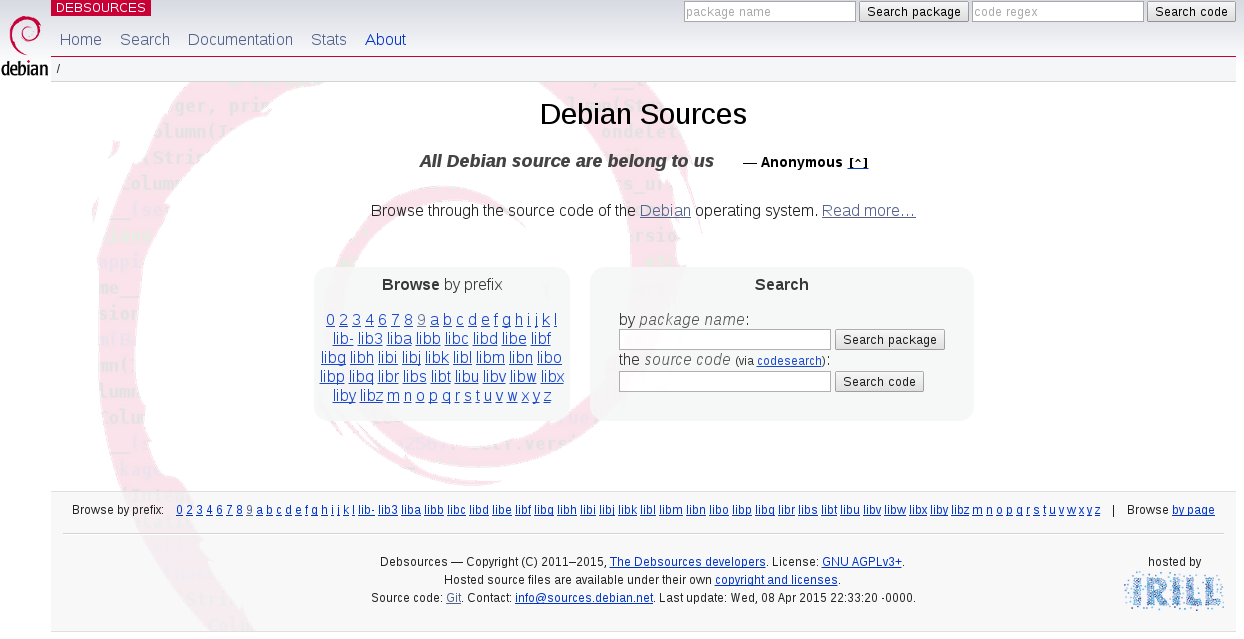
\includegraphics[width=\paperwidth]{img/screenshot-home.png}}
\end{frame}

\begin{frame}
  \frametitle{Source code display}
  \makebox[\textwidth]{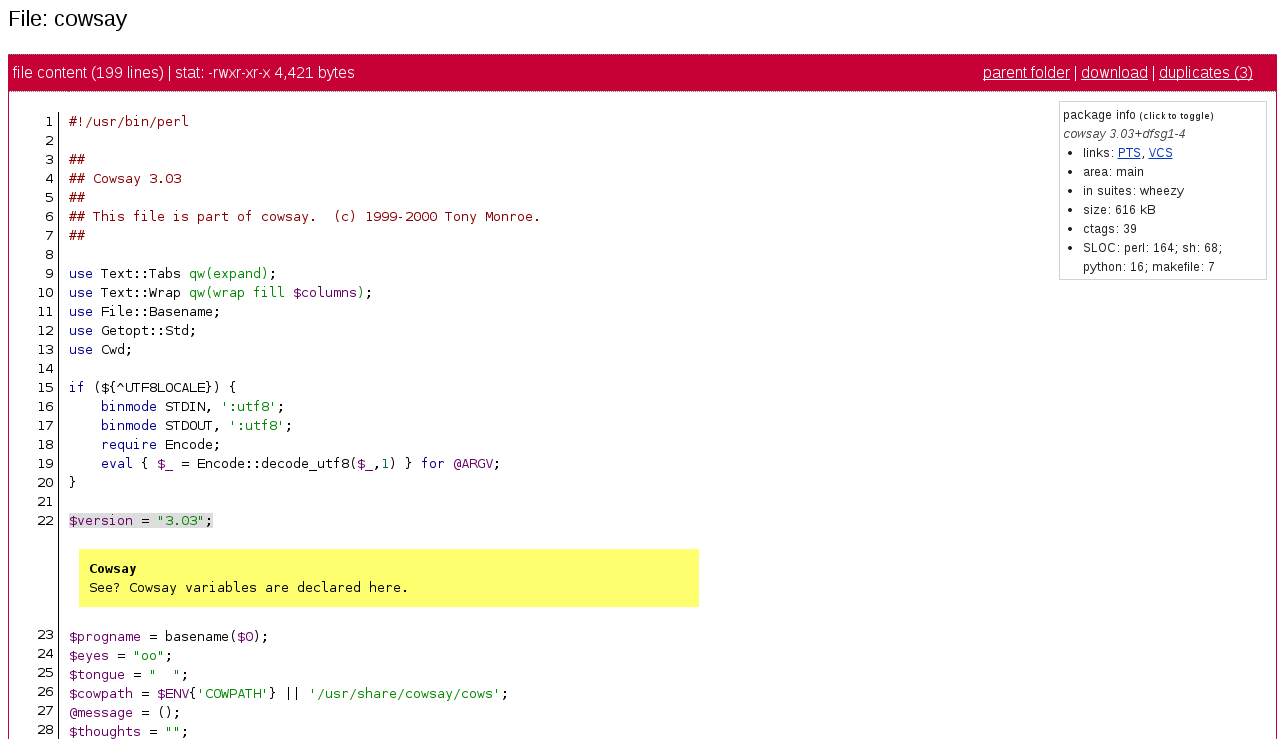
\includegraphics[width=\paperwidth]{img/screenshot-file.png}}
\end{frame}

\begin{frame}
  \frametitle{So what?}
  \framesubtitle{Is this really useful?}
  ``I want to check the source code of \textit{cowsay}. What do?''
  \begin{block}{The old way}
    \texttt{cd /tmp\\
      apt-get source cowsay\\
      cd cowsay-3.03+dfsg1\\
      \ldots\\
      cd ..\\
      rm -r cowsay-3.03+dfsg1
    }
  \end{block}
  \small{Note that it only works on Debian(-based) systems.}
  \pause
  \begin{block}{The new way}
    \texttt{lynx http://sources.debian.net/src/cowsay/}
  \end{block}
  \small{Almost runs on your typewriter.}
\end{frame}

\section{Features}

\subsection{Debsources' features}

\begin{frame}
  \frametitle{Source code browsing}
  \begin{block}{Syntax highlighting}
    For all languages supported by \alert{highlight.js}: C, C++,
    Java, Python, Ruby, Makefile... and 112 others.
  \end{block}
  \pause
  \begin{block}{Included versions}
    Packages in
    \begin{center}
      hamm, slink, potato, woody, sarge, etch, lenny, squeeze, oldoldstable,
      oldstable, stable, testing, unstable, experimental,
      oldoldstable-proposed-updates, oldstable-proposed-updates,
      proposed-updates, testing-proposed-updates, oldoldstable-updates,
      oldstable-updates, stable-updates, wheezy-backports, jessie-backports,
      squeeze-lts
    \end{center}
    are in Debsources.
  \end{block}
\end{frame}

\begin{frame}
  \frametitle{Searching}
  You can search for:
  \begin{itemize}
  \item Packages
  \item Files
  \item File content
    \begin{itemize}
    \item ctags
    \item regular expressions through \texttt{codesearch.debian.net}
    \end{itemize}
  \end{itemize}
  \vfill
  % \pause
  \begin{block}{Content indexing}
    All search data is indexed in Postgres, resulting in pretty decent
    performances (in spite of sub-optimal disk I/O).
  \end{block}
\end{frame}

\begin{frame}
  \frametitle{Advanced search}
  \makebox[\textwidth]{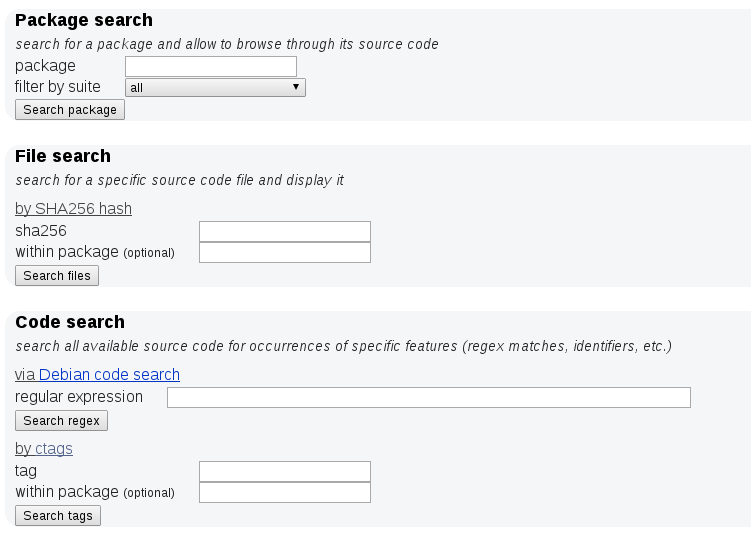
\includegraphics[height=0.8\paperheight]{img/screenshot-search.png}}
\end{frame}

\begin{frame}
  \frametitle{Annotations and highlighting}
  \begin{block}{Use cases}
    \begin{itemize}
    \item I'm a \alert{developer}: \textit{I want to share a pointer to a
        precise location in the source code of package X.}
    \item I'm a \alert{user}: \textit{An errors point me to line 42 in file Y,
        and I look for support on IRC.}
    \item I'm a \alert{static source code checker}: \textit{I found an issue in
        file Z, line 51.}
    \end{itemize}
  \end{block}
\end{frame}

\begin{frame}
  \frametitle{Annotations and highlighting}
  \texttt{http://sources.debian.net/src/\\
    \textbf{package}/\textbf{version}/\textbf{path/to/file.c}?hl=\textbf{a:b}\&msg=\textbf{a:b:c}\#L\textbf{XX}}
  \vspace{1cm}
  % \pause
  \begin{columns}
    \column{.4\textwidth}
    \begin{tabular}{ l l }
      package: & cowsay\\
      version: & 3.03-3\\
      path: & cowsay\\
      highlight: & 32:36\\
      message: & 30:Debian:rocks
      %\\line: & 30
    \end{tabular}
    % \pause
    \column{.6\textwidth}
    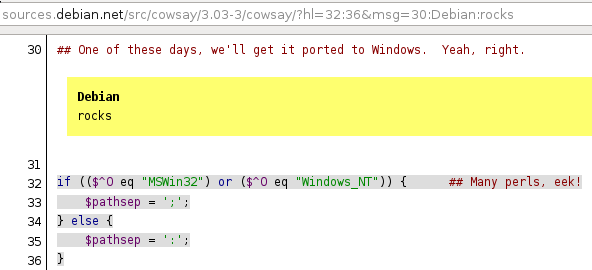
\includegraphics[width=7.5cm]{img/screenshot-hl.png}
  \end{columns}
\end{frame}

\begin{frame}
  \frametitle{Annotations and highlighting}
  \framesubtitle{\alert{Developer}: I want to share a precise
    location in the source code of package X.}
  \makebox[\textwidth]{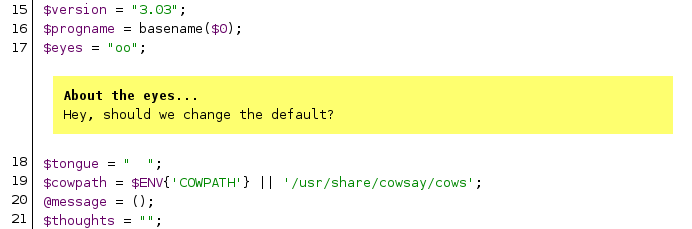
\includegraphics[width=\paperwidth]{img/screenshot-hl1.png}}
\end{frame}

\begin{frame}
  \frametitle{Annotations and highlighting}
  \framesubtitle{\alert{User}: I can't compile software X, it fails
    at line 42 in the file Y.}
  \makebox[\textwidth]{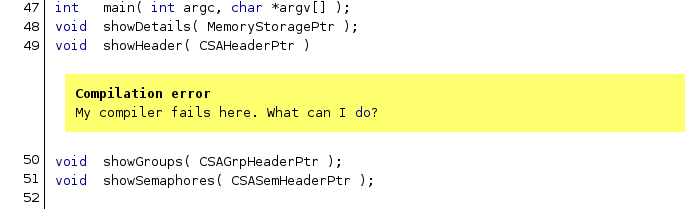
\includegraphics[width=\paperwidth]{img/screenshot-hl2.png}}
\end{frame}

\begin{frame}
  \frametitle{Annotations and highlighting}
  \framesubtitle{\alert{Static analyzer}: I found a semantic error in
    file Y.}
  \makebox[\textwidth]{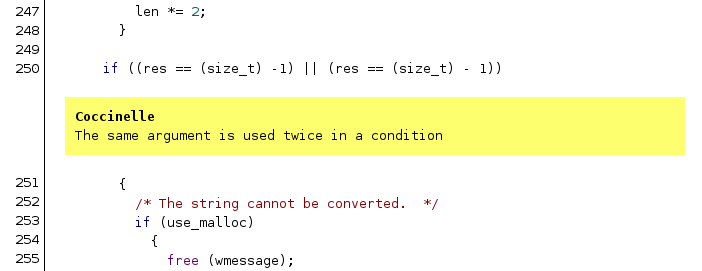
\includegraphics[width=\paperwidth]{img/screenshot-hl3.png}}
\end{frame}

\begin{frame}
  \frametitle{Duplicated files}
  All the files are in the database, along with their checksum.

  The duplicates can be computed, for every file.

  \vspace{1cm}
  \makebox[\textwidth]{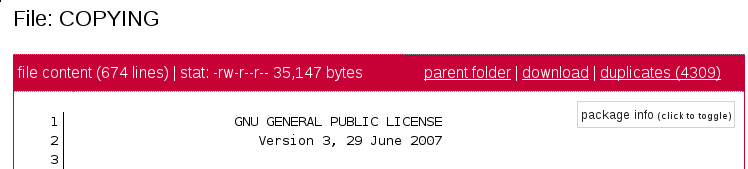
\includegraphics[width=0.9\paperwidth]{img/screenshot-duplicates1.png}}
\end{frame}

\begin{frame}
  \frametitle{Duplicated files}
  \makebox[\textwidth]{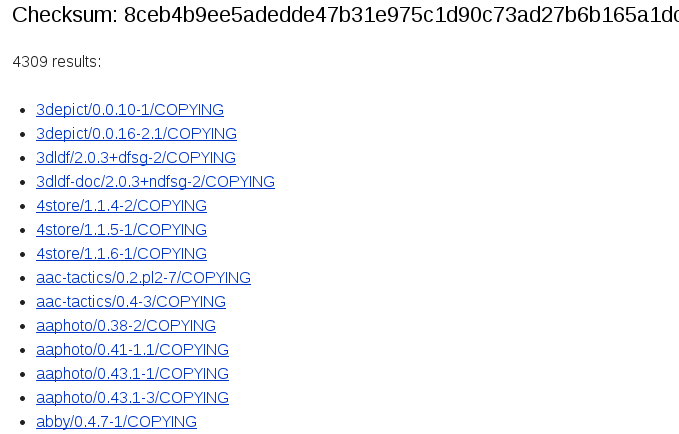
\includegraphics[width=0.9\paperwidth]{img/screenshot-duplicates2.png}}
\end{frame}

\begin{frame}
  \frametitle{Integration in the Debian infrastructure}
  \begin{block}{Codesearch}
    \url{http://codesearch.debian.net} is used for regular expression searches,
    and redirects back to Debsources to consult results.

    Credits: Michael Stapelberg
  \end{block}
  \pause
  \begin{block}{Package tracking systems}
    The old PTS (\url{http://packages.qa.debian.org}) and the new tracker
    (\url{http://tracker.debian.org}) provide links to Debsources (``browse
    source code'').

    Credits: Paul Wise, Raphael Hertzog
  \end{block}
  \pause
  \begin{block}{Need to embed code somewhere?}
    $<$iframe$>$s embedding of files content is supported (see documentation).
  \end{block}
  (or talk to use for more proper integration)
\end{frame}

\begin{frame}
  \frametitle{Statistics}
  \begin{columns}
    \column{.6\textwidth}
    \begin{itemize}
    \item Source code metrics for every package
    \item Plugins: disk size, ctags, sloccount
    \end{itemize}
    \pause
    
    \column{.4\textwidth}
    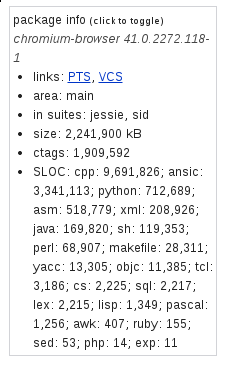
\includegraphics[height=6cm]{img/screenshot-stats.png}
  \end{columns}
\end{frame}

\begin{frame}
  \frametitle{Statistics}
  Aggregated statistics are available at
  \url{http://sources.debian.net/stats/}.
  \begin{block}{Metrics}
    \begin{itemize}
    \item Disk usage
    \item SLOC (source lines of code)
    \item Number of source packages
    \item Number of files
    \item Number of ctags (symbols)
    \end{itemize}
  \end{block}
\end{frame}

\begin{frame}
  \frametitle{Statistics}
  Currently in \textit{sid}:
  \begin{center}
    \begin{tabular}{l|l}
      Source files & 11,787,950 \\
      Source packages & 23,846 \\
      Disk usage & 228,599,736 kB \\
      Ctags & 127,884,129 \\
      Source lines of code & 1,082,453,728 \\
    \end{tabular}
  \end{center}
  \pause
  \begin{enumerate}
  \item C: 439,197,216
  \item C++: 275,342,652
  \item Python: 46,067,009
  \end{enumerate}
  See \url{http://sources.debian.net/stats/sid/} for more
\end{frame}

\begin{frame}
  \frametitle{Statistics}
  \framesubtitle{Fancy graphs}
  \makebox[\textwidth]{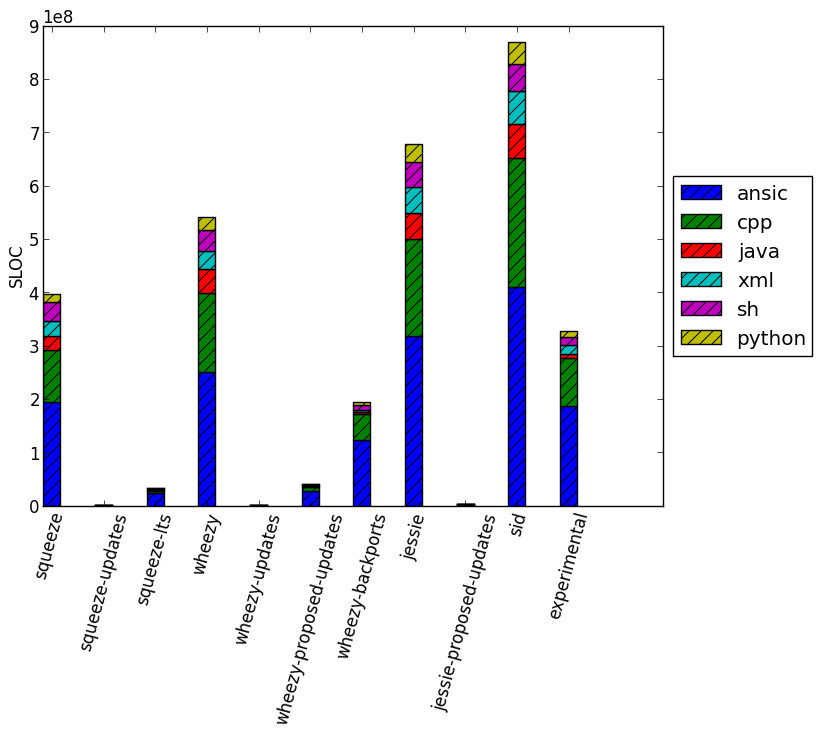
\includegraphics[width=0.7\paperwidth]{img/sloc_bar_plot.png}}
\end{frame}

\begin{frame}
  \frametitle{API}
  All functionalities available via the Web UI, are also available via a
  JSON-based HTTP API:
  % \pause
  \begin{block}{Examples}
    \texttt{\textbf{curl http://sources.debian.net/api/ping/}\\
      \{
        "status": "ok",\\
        ~~"http\_status\_code": 200,\\
        ~~"last\_update": "Mon, 17 Aug 2015 10:43:27 -0000"
      \}}
    \\ ~ \\
    \texttt{\textbf{curl
        http://s.d.n/api/info/package/cowsay/3.03-3/}\\
      \{\\
        "pkg\_infos": \{\\
        ~~  "suites": [\\
        ~~~~      "woody"\\
      ...}
  \end{block}
  Documentation at \url{http://sources.debian.net/doc/api/}.
\end{frame}

\subsection{What's new?}

\begin{frame}
  \frametitle{What's new?}
  \begin{itemize}
    \pause
  \item Many new features since DebConf14
    \pause
  \item Outreachy student: Jingjie Jiang (sophiejjj)
    \pause
  \item GSoC students: Clément Schreiner (clemux), Orestis Ioannou (orestis)
    \pause
  \item Many new contributors:
    \begin{itemize}
      \begin{columns}
        \column{.3\textwidth}
      \item Stefano Zacchiroli: 721
      \item Matthieu Caneill: 483
      \item Orestis Ioannou: 118
      \item sophiejjj: 58
      \item Clément Schreiner: 19
      \item Jason Pleau: 12
      \item Akshita Jha: 7
      \item Jingjie Jiang: 5
        \column{.3\textwidth}
      \item Paul Wise: 1
      \item tessy joseph: 1
      \item sodamatt: 1
      \item Luciano Bello: 1
      \item Christophe Siraut: 1
      \item James McCoy: 1
      \item Tapasweni Pathak: 1
      \end{columns}
    \end{itemize}
  \end{itemize}
\end{frame}

\begin{frame}
  \frametitle{What's new?}
  \framesubtitle{Multiple pop-up messages}
  Credits: Orestis Ioannou and Jason Pleau.\\
  Application: generated code annotations.
  \vspace{7mm}
  ~\\
  \makebox[\textwidth]{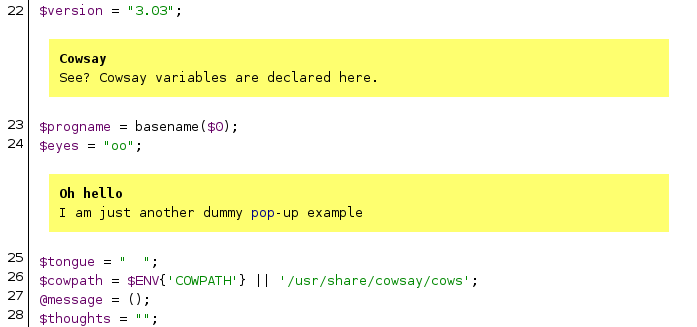
\includegraphics[width=0.9\paperwidth]{img/screenshot-doublepopup.png}}
\end{frame}

\begin{frame}
  \frametitle{What's new?}
  \framesubtitle{Blueprints support}
  Credits: Jingjie Jiang.\\
  Application: new apps plugged.
  \vspace{7mm}
  ~\\  
  \begin{block}{Blueprints}
    \begin{itemize}
    \item Flask apps embedded and plugged together (decentralization)
    \item Implied a big refactoring
    \item Enabled the development of new features (GSoC)
    \end{itemize}
  \end{block}
\end{frame}

\begin{frame}
  \frametitle{What's new?}
  \framesubtitle{Detailed directory listing}
  Credits: Jingjie Jiang
  
  ~\\
  \makebox[\textwidth]{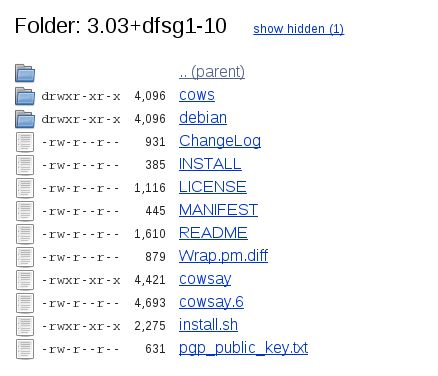
\includegraphics[width=0.6\paperwidth]{img/screenshot-ls.png}}
\end{frame}

\begin{frame}
  \frametitle{What's new?}
  \framesubtitle{File edition in-browser}
  Credits: Raphael Geissert
  
  ~\\
  \begin{block}{File edition}
    A plugin for Iceweasel and Chromium enables the edition of files in
    your browser.

    A patch ready-to-be-sent™ is generated!

    It makes the entire Debian archive editable from a browser.
  \end{block}
\end{frame}

\begin{frame}
  \frametitle{What's new?}
  \framesubtitle{Blueprint app: License information}
  Credits: Orestis Ioannou (GSoC student)

  \begin{block}{debian/copyright}
    Part of the archive uses \alert{machine-readable debian/copyright}
    \pause
    \begin{itemize}
    \item Parse and display this information in the web interface
      \pause
    \item Compute statistics about license usage
      \pause
    \item SPDX (generic license exchange format) export of the
      copyright file
      \pause
    \item API
    \end{itemize}
  \end{block}

\end{frame}

\begin{frame}
  \frametitle{What's new?}
  \framesubtitle{Blueprint app: License information}
  \makebox[\textwidth]{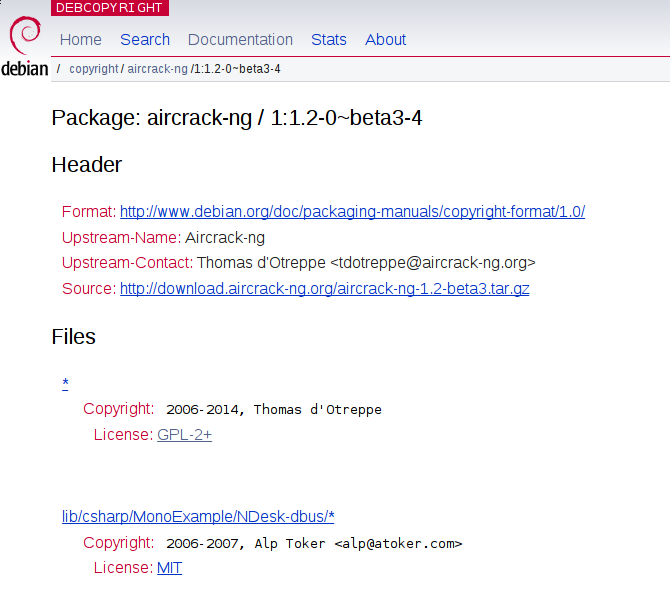
\includegraphics[width=0.7\paperwidth]{img/screenshot-copyright.png}}
\end{frame}

\begin{frame}
  \frametitle{What's new?}
  \framesubtitle{Blueprint app: Patch tracker}
  Credits: Orestis Ioannou (GSoC student)

  \begin{block}{Tracking patches of a package}
    \begin{itemize}
    \item Intended as a replacement of the old patch-tracker
      \pause
    \item Currently supports 3.0 (quilt) format
      \pause
    \item Syntax-highlighting
      \pause
    \item API
    \end{itemize}
  \end{block}
\end{frame}

\begin{frame}
  \frametitle{What's new?}
  \framesubtitle{Blueprint app: Patch tracker}
  \makebox[\textwidth]{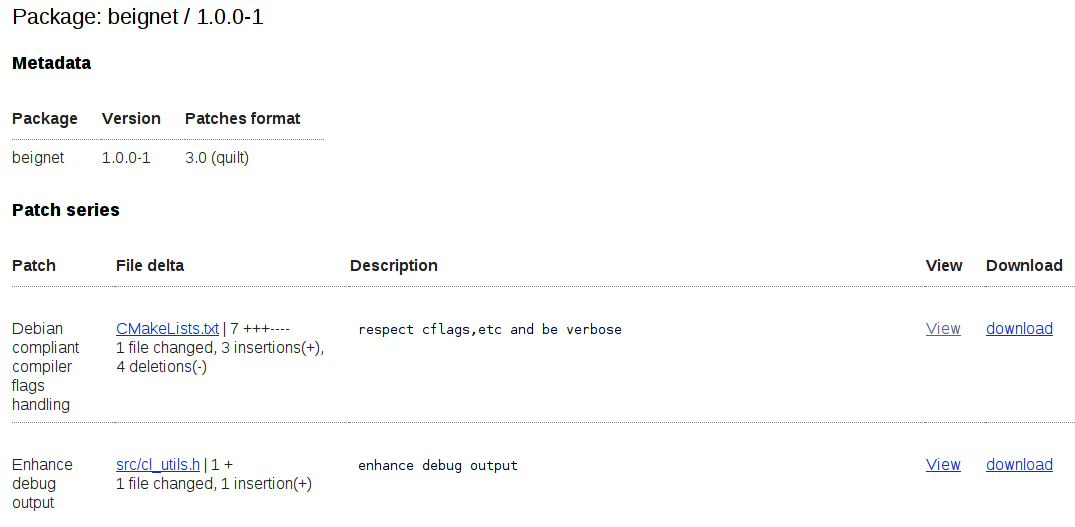
\includegraphics[width=1.0\paperwidth]{img/screenshot-patches.png}}
\end{frame}


\begin{frame}
  \frametitle{What's new?}
  \framesubtitle{Asynchronous updater}
  Credits: Clément Schreiner (GSoC student)

  \begin{block}{Asynchronous updater}
    \begin{itemize}
    \item Rewrite of the stages of the updater (add-package,
      compute-stats, gc, etc)
    \item Using \textit{celery} to spawn independent and asynchronous tasks.
    \end{itemize}
  \end{block}
\end{frame}

\begin{frame}
  \frametitle{For more information about these features}

  \begin{itemize}
  \item Watch the video of the GSoC session (happened earlier this
    afternoon!)
  \item Features soon available at \texttt{sources.debian.net}
    (currently being merged and deployed).
  \end{itemize}
\end{frame}
  
\begin{frame}
  \frametitle{What's new?}
  \framesubtitle{And many many other features...}
  \begin{itemize}
  \item Refactoring
    \pause
    \begin{itemize}
    \item Debsources as a top-level Python module
      \pause
    \item Configuration loader
      \pause
    \item Flake8 compliance (Zack, Jingjie Jiang, and others)
      \pause
    \end{itemize}
  \item Test coverage (Jingjie Jiang, Clément Schreiner, and others)
    \pause
    \begin{itemize}
    \item 84\% now!
    \end{itemize}
    \pause
  \item Case-insensitive package name search (Akshita Jha)
    \pause
  \item Better statistics charts (Orestis Ioannou)
    \pause
  \item Python3 support (Zack)
  \end{itemize}
\end{frame}

\subsection{Roadmap}

\begin{frame}
  \frametitle{Roadmap}
  \begin{block}{Static analysis}
    \begin{itemize}
      \item Automatic runs of static analysis tools (e.g. clang,
        coccinelle) on all Debian packages
      \item Statistics gathering on bugs evolution
      \item $\to$ Debile, Firewoes
    \end{itemize}
  \end{block}
\end{frame}

\begin{frame}
  \frametitle{Roadmap}
  \framesubtitle{And many smaller items}
  \begin{itemize}
  \item more live statistics (about licenses, patches, etc)
    \pause
  \item file name search
    \pause
  \item binary package $\to$ source package redirection
    \pause
  \item tarball-in-tarball support
    \pause
  \item 100\% test suite coverage (one day...)
    \pause
  \item file-level deduplication
    \begin{itemize}
    \item \lstinline[style=sql]{select count(*) from checksums;}
      \hfill $\rightarrow$ 35'370'653
    \item
      \lstinline[style=sql]{select count(distinct sha256) from
        checksums;}
      \hfill $\rightarrow$ 15'822'745
    \item[] \hfill $\Rightarrow$ \alert{deduplicated core:
      $\approx$ 45\%}
    \end{itemize}
  \end{itemize}
\end{frame}

\section{Technologies}

\begin{frame}
  \frametitle{Technologies}
  \framesubtitle{What languages and technologies do we use?}
  \begin{itemize}
  \item \textbf{Code base}: (almost) entirely in Python
    \pause
  \item \textbf{Web application}: Flask framework, Jinja2 templates,
    HTML/CSS/Javascript
    \pause
  \item \textbf{Database}: PostgreSQL
    \pause
  \item Apache web server, SQLAlchemy, ...
  \end{itemize}
\end{frame}

\begin{frame}
  \frametitle{Overview}
  \framesubtitle{Architecture}
  \begin{center}
    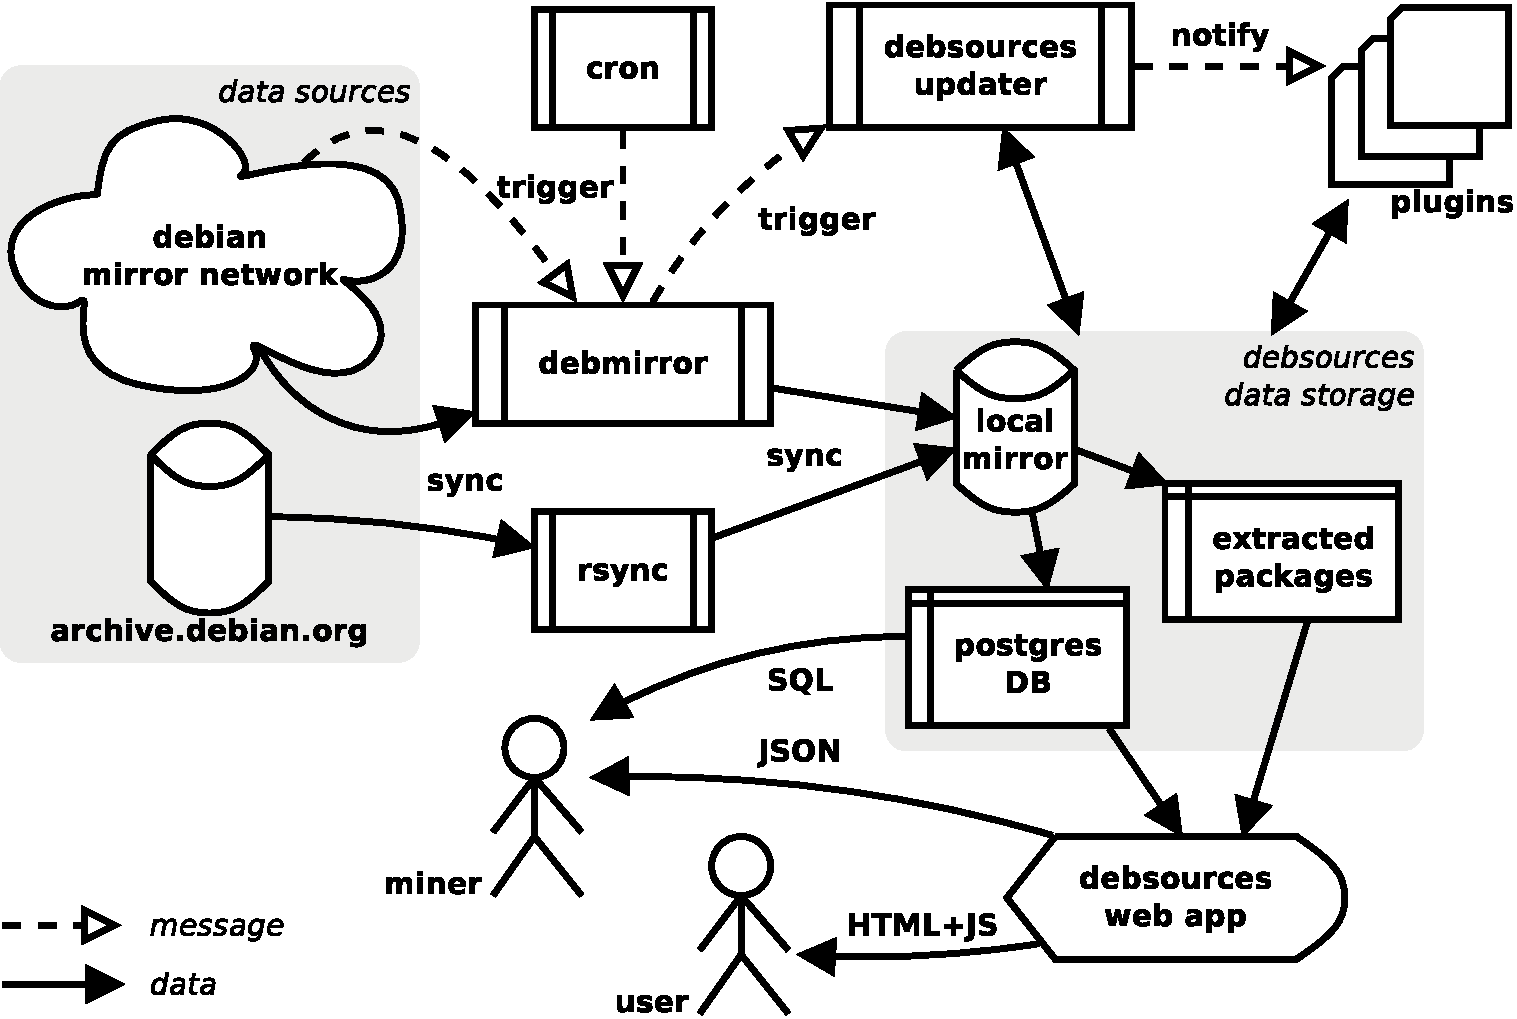
\includegraphics[width=0.9\textwidth]{img/architecture}
  \end{center}
\end{frame}

\begin{frame}
  \frametitle{Overview}
%  \framesubtitle{Database and plugins}
  ~\hfill {\small data model (excerpt)}
  \vspace{-0.5cm}
  \begin{center}
    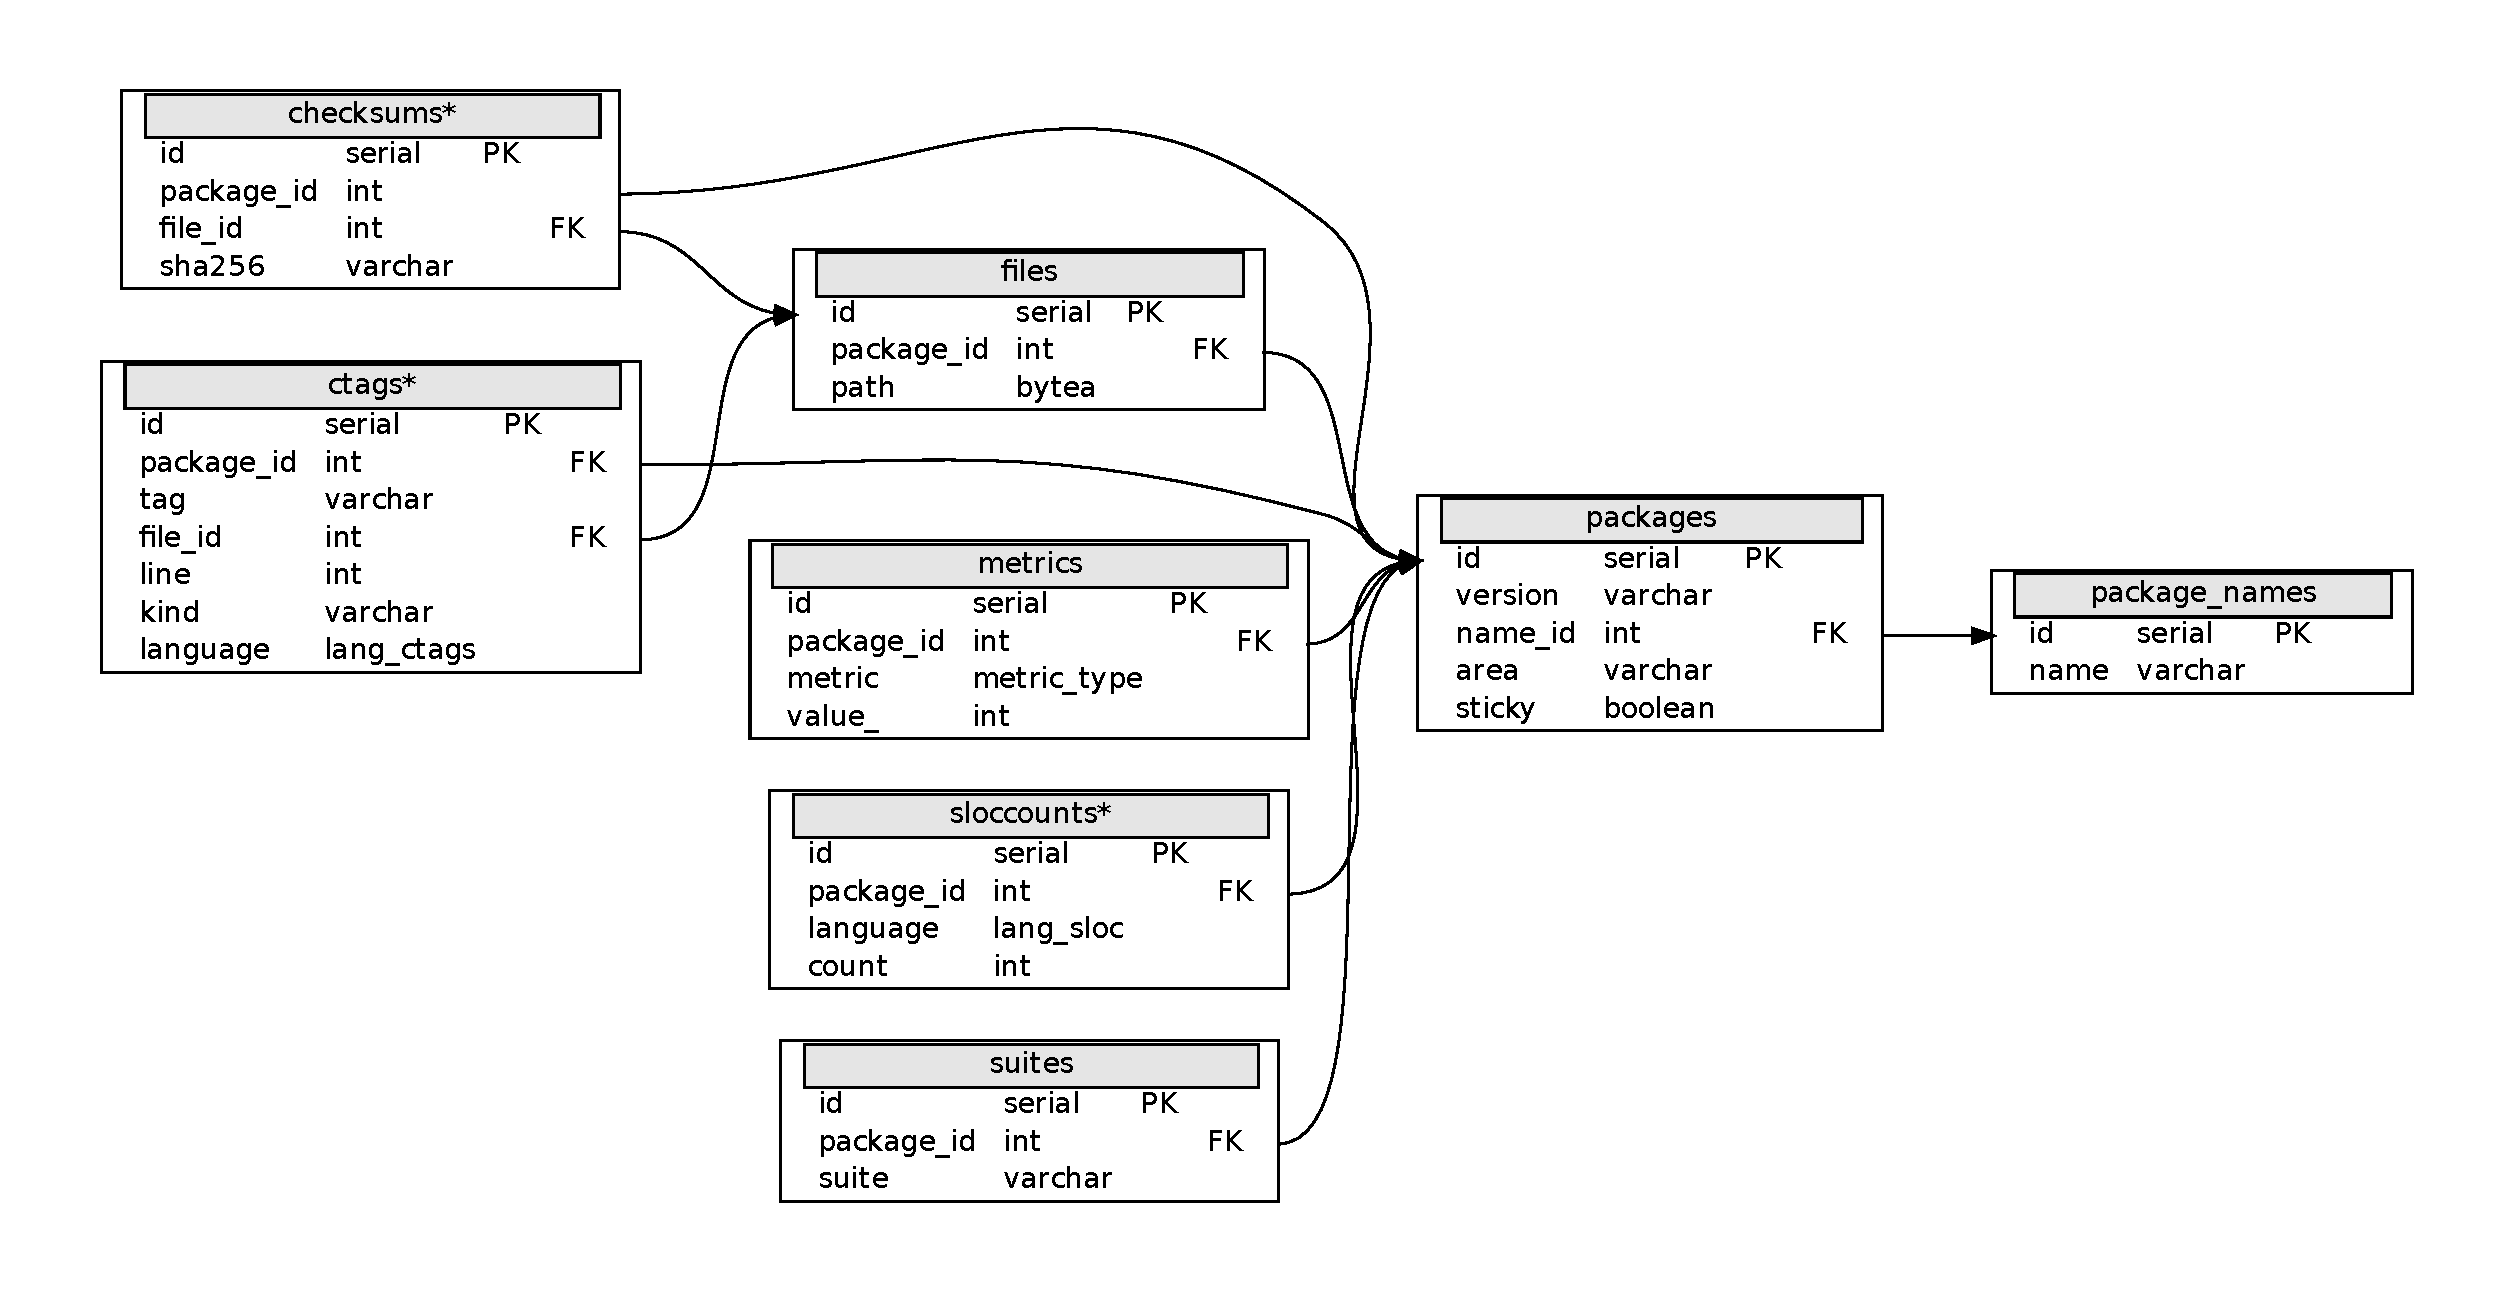
\includegraphics[width=\textwidth]{img/dbschema-simpl2}
  \end{center}
  \vspace{-2.8cm}
  \begin{center}
    \footnotesize
    ~\hspace{6.5cm}
    \begin{tabular}{@{}l|r@{}}
      \multicolumn{1}{c|}{\textbf{table}}
      & \multicolumn{1}{c}{\textbf{rows}\footnote{snapshot, 31
          July 2014}} \\
      \hline
      suites\_info   &          16 \\
      \hline
      package\_names &      29,286 \\
      (source) packages &   83,597 \\
      suites (mapping) &   120,550 \\
      \hline
      metrics (e.g., \texttt{du})
      &      83,597 \\
      sloccounts    &     298,360 \\
      checksums     &  35,370,653 \\
      ctags         & 358,773,259 \\
    \end{tabular}
  \end{center}
\end{frame}

\begin{frame}{Disk usage}
  \begin{columns}
    \begin{column}{0.5\textwidth}
      \begin{itemize}
      \item unpacked sources: \hfill 805 GB
        \note[item]{this is without any deduplication; I'll
          get back to that}
      \item PostgreSQL DB: \hfill 145 GB
      \item Source mirror: \hfill 135 GB
      \end{itemize}
      \alert{Hosting requirements}: \hfill $\approx$ 1.1
      TB\\[1ex]
      ~\hfill {\footnotesize (17 August 2015)}
    \end{column}
    \pause
    \begin{column}{0.5\textwidth}
      \begin{figure}
        \centering
        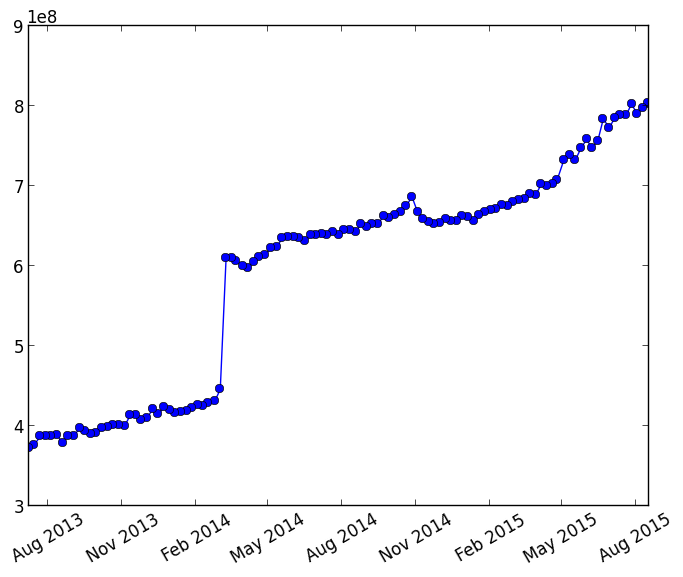
\includegraphics[width=\textwidth]{img/disk-usage}
        \caption{unpacked sources trend (peek due to
          \texttt{archive.d.o}
          injection)}
      \end{figure}
    \end{column}
  \end{columns}
\end{frame}

\section{Research platform}

\begin{frame}
  \frametitle{Research platform}
  \begin{block}{Facts}
    \begin{itemize}
    \item Debsources is a \alert{huge} software collection.
    \item Homogeneous: all software follow Debian's packaging format.
    \item It is up-to-date.
    \end{itemize}
  \end{block}
  \pause
  
  \begin{block}{Software evolution}
    \begin{itemize}
    \item 20 years of source code evolution.
    \item Plugins to compute stats.
    \end{itemize}
  \end{block}
  \pause
  
  \alert{Nice charts can be computed with this!}

  Example: What are the trending programming languages?
\end{frame}

\begin{frame}
  \frametitle{Research platform}
  \framesubtitle{Software metrics evolution over Debian releases}
  \vspace{-0.3cm}
  \begin{figure}
    \centering
    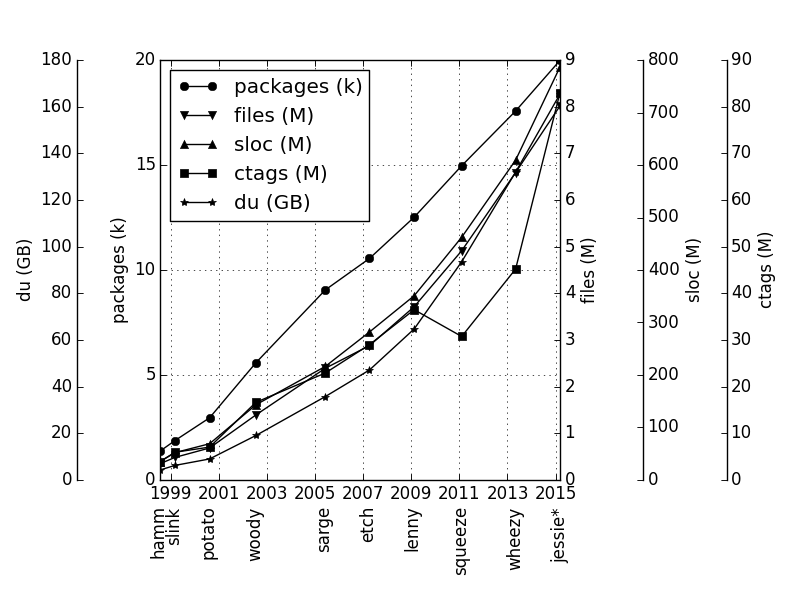
\includegraphics[width=0.85\textwidth]{img/size-combined}
    %\caption{}
  \end{figure}
\end{frame}

\begin{frame}
  \frametitle{Research platform}
  \framesubtitle{File size per language, evolution over Debian releases}
  \vspace{-0.3cm}
  \begin{figure}
    \centering
    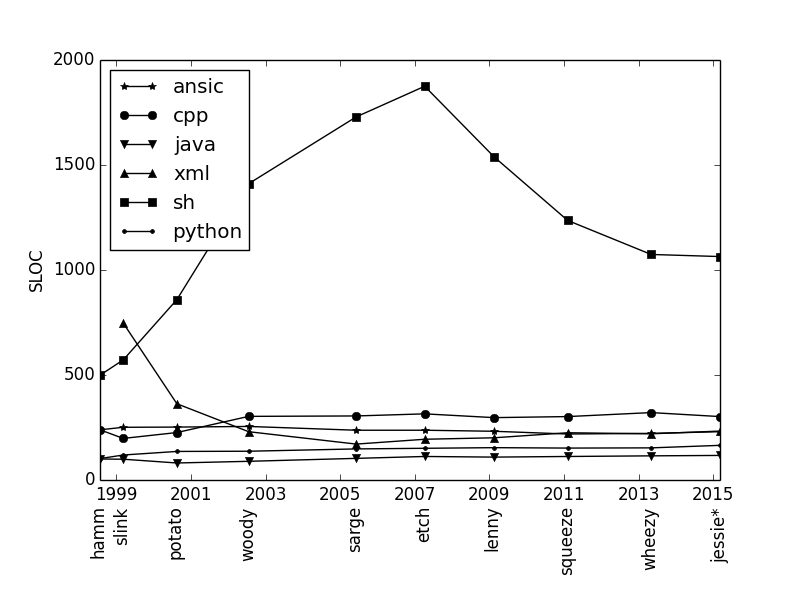
\includegraphics[width=0.85\textwidth]{img/size-file-per-language}
    %\caption{}
  \end{figure}
\end{frame}

\begin{frame}
  \frametitle{Research platform}
  \framesubtitle{Absolute evolution of SLOC per language, over Debian releases}
  \vspace{-0.3cm}
  \begin{figure}
    \centering
    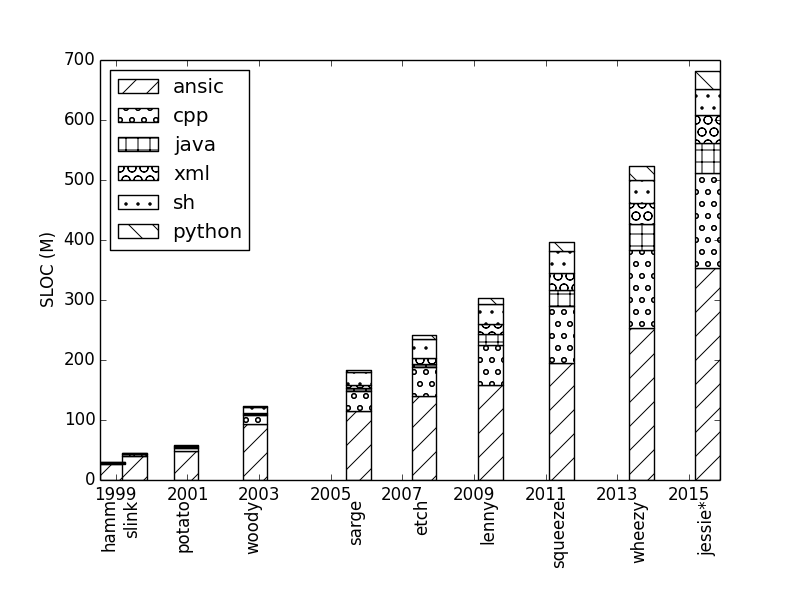
\includegraphics[width=0.85\textwidth]{img/sloc-evol-abs}
    %\caption{}
  \end{figure}
\end{frame}

\begin{frame}
  \frametitle{Research platform}
  \framesubtitle{Relative evolution of SLOC per language, over Debian releases}
  \vspace{-0.3cm}
  \begin{figure}
    \centering
    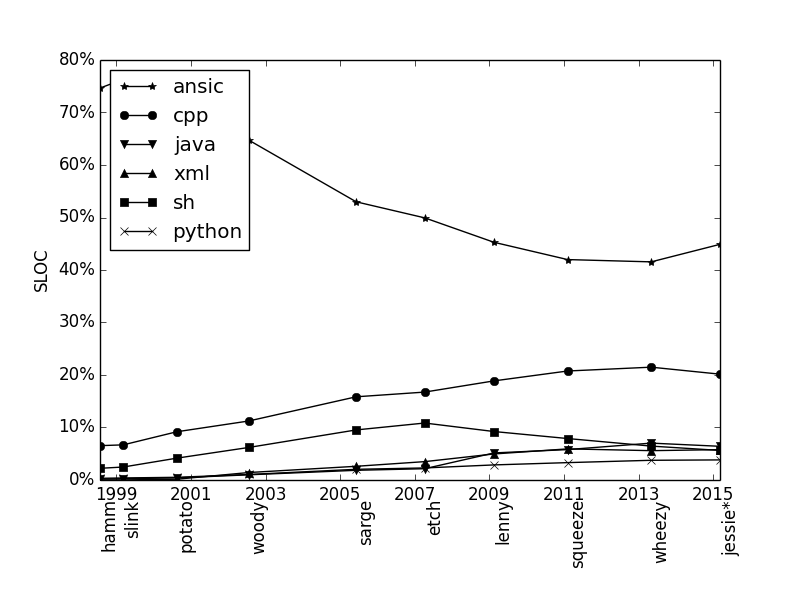
\includegraphics[width=0.85\textwidth]{img/sloc-evol-rel}
    %\caption{}
  \end{figure}
\end{frame}

\begin{frame}
  \frametitle{Research platform}
  \framesubtitle{Publications}
  \begin{itemize}
    \item Matthieu Caneill, Stefano Zacchiroli. \textbf{Debsources:
      Live and Historical Views on Macro-Level Software Evolution.} In
      proceedings of ESEM 2014: 8th International Symposium on
      Empirical Software Engineering and Measurement.
    \item Stefano Zacchiroli. \textbf{The Debsources Dataset: Two
      Decades of Debian Source Code Metadata.} To appear in
      proceedings of MSR 2015: The 12th Working Conference on Mining
      Software Repositories.
  \end{itemize}
  \vspace{1cm}
  \small{You can find the PDFs of the articles on \url{http://sources.debian.net/doc/}.}
\end{frame}

\section{Hacking}

\begin{frame}
  \frametitle{Hacking}
  \framesubtitle{How can I contribute?}
  \begin{block}{Step 1: clone Debsources git repository}
    \texttt{git clone git://anonscm.debian.org/qa/debsources.git}
  \end{block}
  \pause
  \begin{block}{Step 2: Set-up a development environment}
    \begin{itemize}
    \item Follow the instructions in the \alert{HACKING} file,
    \item Or use Docker!
      \texttt{bin/debsources-docker-build \&\& bin/debsources-docker-run}
      will setup a \alert{Docker container} with all batteries included:
      dependencies, database, test data, configuration.
    \end{itemize}
  \end{block}
  \pause
  \begin{block}{Step 3: open your editor and hack!}
    \alert{Bugs list}:
    \url{https://bugs.debian.org/cgi-bin/pkgreport.cgi?pkg=qa.debian.org;tag=debsources}
    \\
    or: implement your own \alert{plugin} (see examples), add \alert{features}, etc.
  \end{block}
\end{frame}

\background

\begin{frame}[plain]
  \center{
    {\huge Thanks!}
    {\huge Questions?}\\
    \vspace{1.5cm}
    {\Large Stefano Zacchiroli, Matthieu Caneill}\\
    \texttt{info@sources.debian.net}\\
    \vspace{1.5cm}
           {\small Slides: Licensed CC-BY-SA.\\
             \url{http://upsilon.cc/~zack/talks/2015/20150818-dc15-debsources.pdf}}
  }
\end{frame}

\end{document}
